\documentclass[laboratorio]{guia}

\def \practnum {1} 
\def \practica {Electrost\'atica}

\def \materia {Laboratorio de F\'\i sica II para Qu\'\i micos}
\def \periodo {2do. Cuatrimestre de 2015}
\def \catedra {Pablo Cobelli}
\def \website {http://materias.df.uba.ar/f2qa2015c2}
 
\usepackage{graphics}
\usepackage{amsmath}
\usepackage{amsfonts}
\usepackage{graphicx}
\usepackage{float}
\usepackage{wrapfig}
\usepackage{subfigure}
\usepackage{bm}
\usepackage{grffile}
\usepackage{color}
\usepackage{framed}
\usepackage[utf8]{inputenc}
\usepackage[T1]{fontenc}
\usepackage{lmodern}
\usepackage{circuitikz}
\usepackage[spanish]{babel}
\usepackage{babelbib}
\selectbiblanguage{spanish}

 
% 
%----------------------------------------------------------
% Agrega al path de figuras el subdirectorio con el mismo
%     nombre que el archivo principal del proyecto
\graphicspath{{./\jobname/}}

%----------------------------------------------------------
% Definicion del entorno 'sabermas'
\makeatletter
\definecolor{shadecolor}{rgb}{0.89,0.91,0.94}
\newenvironment{sabermas}[1]{%
\vfill
\begin{shaded}
  \begin{center}
  {\textsection{Para saber m\'as}}
  \end{center}
  #1
\sf } 
{%
\end{shaded}%
}
\makeatother

%----------------------------------------------------------
% Definicion del entorno 'problema'
\newcounter{ContadorProblema}
\setcounter{ContadorProblema}{0}
\newcounter{TieneFiguraAsociada}
\setcounter{TieneFiguraAsociada}{0}
\newcounter{UbicacionFigura}
\setcounter{UbicacionFigura}{0}

\newenvironment{problema}[2][]
{%
    \ifx\relax#1\relax%
        \setcounter{TieneFiguraAsociada}{0}
        \else
        \setcounter{TieneFiguraAsociada}{1}
    \fi
    \def \archivofigura {#1}
    % 
    \refstepcounter{ContadorProblema}
    \noindent%
    \ifnum\value{TieneFiguraAsociada} < 1%
        {\sffamily \bfseries Problema \arabic{ContadorProblema}.}
        %{\sc {#1}}%
        \par\nobreak\par\nobreak%
        \medskip 
    \else
        % Va con figura; resta determinar de que lado.
        \ifnum\value{UbicacionFigura} < 1
            % Poner la figura del lado derecho
            \begin{minipage}{12.25cm}
            {\sffamily \bfseries Problema \arabic{ContadorProblema}.}
            %{\sc {#1}}%
            \par\nobreak\par\nobreak%
            \medskip 
        \else
            % Poner la figura del lado izquierdo
            \begin{minipage}{4.5cm}
                \centering
                \includegraphics[width=4.5cm]{\archivofigura}
                {\footnotesize {\sffamily Esquema asociado al 
                problema \arabic{ContadorProblema}}.}
            \end{minipage}\hfill%
            \begin{minipage}{12.25cm}
                {\sffamily \bfseries Problema \arabic{ContadorProblema}.}
                %{\sc {#1}}%
                \par\nobreak\par\nobreak%
                \medskip 
        \fi
    \fi
}
{%
    \ifnum\value{TieneFiguraAsociada} < 1%
        % \par \bigskip \vskip 0.3cm
    \else
        % Va con figura; resta determinar de que lado.
        \ifnum\value{UbicacionFigura} < 1
            % Poner la figura del lado derecho
            \end{minipage}\hfill%
            \begin{minipage}{4.5cm}
                \centering
                \includegraphics[width=4.5cm]{\archivofigura}
                {\footnotesize {\sffamily Esquema asociado al 
                problema \arabic{ContadorProblema}}.}
            \end{minipage}
        \else
            % Poner la figura del lado izquierdo
            \end{minipage}%
        \fi
    \fi
    \setcounter{TieneFiguraAsociada}{0}
    \par \bigskip \vskip 0.3cm
    % Permutamos el valor de la ubicacion
    \ifnum\value{UbicacionFigura} < 1
        \setcounter{UbicacionFigura}{1}
    \else
        \setcounter{UbicacionFigura}{0}
    \fi
}

%----------------------------------------------------------
% Definicion/Redefinicion de estilos
\renewcommand{\vec}[1]{\ensuremath{\mathbf{#1}}}



\hyphenation{ coe-fi-cien-tes coe-fi-cien-te au-to-va-lor
              au-to-va-lo-res co-rres-pon-der pro-ble-ma 
              cual-quie-ra po-la-ri-za-cio-nes }

\graphicspath{{./electrostatica/}}

\begin{document} 
\objetivo{
  Dibujar mapas de líneas o superficies equipotenciales, es decir, del conjunto de puntos en el espacio que se encuentran caracterizados por un mismo valor del potencial eléctrico \(V\) para distintas configuraciones de electrodos conectados a una fuente de baja tensión e inmersos en un medio líquido poco conductor.
  \tematicas{Electrostática, potencial electrostático, campo eléctrico, conductores y dieléctricos.}
} 
\maketitle


\section{Campo y potencial eléctrico}
Toda fuerza aplicada a lo largo de una trayectoria entre los puntos en el \(\va{r}_1\) y \(\va{r}_2\) está haciendo un trabajo
\begin{equation} 
  W_{12}= \int_1^2 \va{F} \va{\dd{r}},
\end{equation}
y todo trabajo de una fuerza conservativa se corresponde con el negativo de una variación de una energía potencial.
Un ejemplo de esto es el de la fuerza peso \(\va{P}= m \va{g}\), en cuyo caso la energía potencial es la gravitatoria
% y todo trabajo de una fuerza conservativa, como el la eléctrica, se corresponde con el negativo de una variación de una energía potencial, en este caso eléctrica
\begin{equation} 
  W_{peso\,12}= \int_1^2 m\va{g} \va{\dd{r}}= - \Delta E_\text{pot. grav.}= m g (h_2 - h_1), 
  % W_{12}= - \Delta E_\text{eléctrica}. 
  \label{travail}
\end{equation}
donde \(h_2\) y \(h_1\) son dos alturas siendo la primera mayor, siempre y cuando consideremos que el campo gravitatorio \(\va{g}\) no varia entre esas dos alturas.

Ahora presentaremos otras fuerza conservativa, la electrostática.
En lugar de \(m\) ubicaremos una carga de prueba \(q\), y en lugar del campo gravitatorio \(\va{g}\) tendremos un campo campo eléctrico \(\va{E}\).
Este último ejerce sobre \(q\) una fuerza
\begin{equation} 
  \va{F} = q \: \va{E}.
  \label{forza}
\end{equation}
Como la fuerza \(\va{F}\) es un vector y la carga eléctrica \(q\) un escalar, resulta
claro que el campo eléctrico local \(\vec{E}\) es también un vector. 

El trabajo de esta fuerza se calcula igual que en (\ref{travail})
\begin{equation} 
  W_{elec.\,12}= \int_1^2 q \va{E} \va{\dd{r}}= - \Delta E_\text{elec.}.
  \label{travailElect}
\end{equation}
Es útil independizarse de la magnitud de la carga de prueba \(q\) para describir la variación de la energía, por lo que se acostumbra definir
\begin{equation} 
  \frac{W_{elec.\,12}}{q}= \int_1^2 \va{E} \va{\dd{r}}= - \Delta V,
  \label{travailElect}
\end{equation}
donde \(V\) recibe el nombre de potencial eléctrico.
Y así como $W_{12}$ el trabajo que tenemos que realizar para llevar la carga $q$ desde el punto 1 al punto 2 $W_{12}$ es una magnitud escalar, el potencial también lo es.

Así como podemos invertir la relación (\ref{travail}) y puede obtenerse \(\va{P}\) como el gradiente de la \(E_\text{gravitatoria}\), es decir \(\va{P}= - \grad E_\text{gravitatoria}\), esto mismo se aplica a cualquier fuerza conservativa, como la electrostática
\begin{equation} 
  \va{F}_\text{elec.}= - \grad E_\text{elec.} = - q \grad V.
\end{equation}
Y como vimos en la expresión (\ref{forza}) la relación de esta fuerza con \(\va{E}\) es claro que las componentes del campo eléctrico pueden expresarse en función del potencial eléctrico:
\begin{equation}
    \vec{E} = - \vec{\nabla} V,
\end{equation}
expresión que resulta válida en cualquier sistema de coordenadas. 

Y así como sin nos moviamos perpendiculares a \(\va{g}\) la componente de \(\va{P}\) en esa dirección era nula, es decir si manteníamos a la misma altura manteniamos la misma \(E_\text{pot. grav.}\), si nos movemos un una línea donde el potencial eléctrico es constante, $\Delta V=0$ (línea equipotencial), la componente de $\va{E}$ sobre esta línea es nula.
En otras palabras, $\va{E}$ es siempre perpendicular a las líneas (o, más generalmente, superficies) equipotenciales.

La idea central de este experimento consiste en determinar experimentalmente, para una dada configuración, las líneas equipotenciales (es decir, las líneas sobre las cuales el potencial es constante).
A partir de estas líneas equipotenciales, se pueden luego hallar las líneas de campo $\va{E}$, trazando líneas perpendiculares a las equipotenciales.


\section{Dispositivo experimental}
Las mediciones se realizaran en una bandeja de vidrio o acrílico transparente, de aproximadamente \(30 \times 20 \times \SI{4}{\centi\metre}\), que debe contener la mínima cantidad de agua de red que alcance a cubrir toda la base de la bandeja. 
Dos placas metálicas (de cobre, bronce y/o aluminio) se dispondrán parcialmente inmersas en el líquido como muestra la figura \ref{fig:1}.
Dos cables banana-cocodrilo conectarán las placas a una una fuente de tensión alterna de \num{5}-\SI{15}{\volt}, que les impondrá una diferencia de potencial entre ambas.
Se utiliza alterna con el fin de minimizar la degradación por electrólisis de los metales.
Finalmente, a fin de determinar el valor del potencial en un punto dado del espacio, se hará uso de un voltímetro.
Un cable banana-cocodrilo conectará el puerto común del multímetro a una de las placas y un cable de prueba (banana-punta) se conectará al puerto marcado con ``V''.
\begin{figure}[ht!]
  \centering
    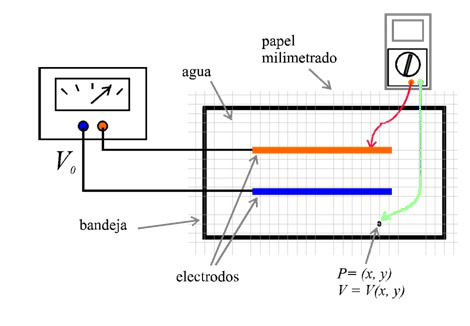
\includegraphics[width=8.5cm]{LG01--000.png}
    \caption{Esquema del dispositivo experimental propuesto (bandeja en vista superior).
	  La bandeja de material aislante contiene agua. Las líneas gruesas continuas representan los electrodos metálicos.
	  En el punto de coordenadas \((x,y)\), se mide el valor del potencial eléctrico \(V(x,y)\).}
    \label{fig:1}
\end{figure}



\section{Análisis exploratorio semi-cuantitativo}
Para explorar cómo se comporta el sistema use el multímetro en modo voltímetro en una escala acorde al ajuste de la fuente y ``pinche'' con la punta de prueba en diversos puntos de la bandeja. 
Después de verificar que la indicación del multímetro es coherente con sus expectativas (¿Donde el potencial es mayor?) deberá realizar las tres siguientes actividades:
\begin{enumerate}
    \item Determine las líneas equipotenciales en toda la bandeja siguiendo el procedimiento que se indica a continuación.
    \item Sin mover los electrodos, coloque un conductor entre ellos.
        Determine las líneas equipotenciales de este nuevo arreglo (ver figura \ref{fig:2}).
		En particular interesa estudiar la forma de las líneas equipotenciales alrededor del conductor, por lo que no dude en aumentar la ``densidad'' de puntos medidos a su alrededor.
		¿Cómo deberían ser las líneas equipotenciales dentro del mismo? No solo lo imagine, ¡mídalo!
    \item Repita el punto anterior pero usando un aislante en vez del conductor.
\end{enumerate}


\begin{figure}[ht!]
  \centering
    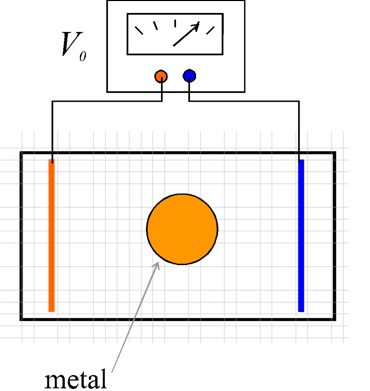
\includegraphics[width=5cm]{LG01--001.png}
    \caption{Esquema del segundo dispositivo experimental propuesto (bandeja en vista superior). 
      Los electrodos metálicos se alejan entre sí para disponer entre los cuales un medio conductor de forma geométrica simple. 
    }
    \label{fig:2}
\end{figure}


\subsection{Procedimiento para determinar equipotenciales}
\begin{enumerate}
  \item Debe intentar medir por lo menos 6 a 8 puntos para cada equipotencial.
  Para esto basta con muestrear la superficie de la bandeja en puntos regularmente distribuido con separaciones de \SI{2}{\centi\metre}.
  Imaginando un sistema de coordenadas ayudado por el papel milimetrado, ordene sus mediciones como una matriz.
    Para ayudarse utilizará el programa Matlab\textsuperscript{\textregistered}, o su homólogo de código abierto GNU Octave.
	\begin{enumerate}
      \item Cree una matriz con el nombre que quiera (por ej. \verb'potenciales') y anote sus mediciones en la fila y columna correspondiente con el sistema de coordenadas elegido.
    Ambos programas proveen la función \verb'contourf' que traza líneas uniendo los valores que serían iguales interpolando entre los datos de la matriz.
      En el caso de las mediciones de potencial \(V\) tales líneas corresponden a las equipotenciales.
    Estas son las líneas equipotenciales correspondientes a la geometría de electrodos (o electrodos y conductor o aislante) elegida.
	  \item Para cada configuración intente de que alguna de ellas se encuentren cerca de cada electrodo y algunas en las zonas centrales del arreglo.
    Esto lo puede lograr variando el parámetro de cuantas líneas debe dibujar la función, por ej. ejecutando el comando \verb'contourf(potenciales,15)' donde \num{15} es el número de líneas.
      \item Finalmente ejecute \verb'colorbar' para que figure la escala de \(V\) en el gráfico generado, y grabe tanto la matriz como el gráfico.
	\end{enumerate}
  \item Para el caso del conductor entre los electrodos, analice la configuración de líneas equipotenciales alrededor del conductor.
        ¿Cómo son las líneas de campo sobre la superficie del conductor?
    Tenga la precaución de utilizar otro nombre para la matriz en el programa para no sobre escribir los datos de la medición anterior.
    Grafique y grabe sus datos.
  \item Preste particular atención a la configuración en la que se
        dispone un aislante entre los electrodos. En particular estudie las
        líneas equipotenciales alrededor del aislante. ¿Cómo son las
        líneas de campo y el campo mismo sobre su superficie? ¿Cómo
        puede explicar lo que observa en este caso?
\end{enumerate}


\nocite{Alonso1998,Purcell1988,Reitz1996,Trelles1984}
\bibliographystyle{unsrt} 
\bibliography{Bibliografia}

\end{document}
